\chapter{The sequential coalescent and coalescent hidden Markov models}
\label{chap:smc-coalhmm}

Coalescence theory provides a very powerful framework for genetics modelling and inference, and the coalescence process with recombination underlies many important analysis tools. Drawing inference from sequences with recombination, however, often involves integrating over all possible ancestries, modelled as the so-called ancestral recombination graph (ARG), a process that rarely scales to more than a few, short sequences due to the complexity and state space size of the ARG. To alleviate this, the \emph{sequential Markov coalescence} approximation assumes that statistical dependencies between local genealogies are Markov~\cite{McVean:2005ho, Marjoram:2006hp,Hobolth:2014cw}.

In this chapter, I give a short introduction to the essentials of coalescence theory and coalescent hidden Markov models. In the following chapters I will then describe a framework for semi-automatically constructing CoalHMMs for various demographic models.

\section{Coalescence processes}

Coalescence theory~\cite{Hein:2005vz} describes the ancestry of a sample of present day genes and gives probabilities to all the possible genealogies that could have created the variation seen in the samples. The typical description of the coalescence model is as a continuous time Markov process running backwards in time, describing the various events that could have occurred in the past.

When not considering recombinations this process simply models how the samples find common ancestors, where lineages stretching backwards in time coalesce into fewer and fewer ancestral lineages.  An outcome of such a process is a tree-genealogy where inner nodes correspond to where two lineages find their most recent common ancestor. The time-depths of these nodes, and thus the branch lengths of the tree, are given by the rate of coalescence, a parameter that is determined by the size of the population the samples are taken from (the so-called ``effective population size'', $2N_e$, or its mutation-scaled version $\theta=4 N_e \mu$, see \citet{Hein:2005vz}).

In the simplest version of the coalescence process, a pair of sampled genes coalesce at a fixed rate, $c$, (typically parameterised by the effective population size where the rate is then $c=2/\theta$). The probability density for the time at which they coalesce is therefore exponentially distributed with this rate. When more than two samples are considered, each pair---of which there are $n \choose 2$ possible---coalesce at this rate and thus the density for the first coalescence event is $c{n \choose 2}$. At the first coalescence event a random pair is merged---the samples, or lineages, are said to find a common ancestor---and the process continues back in time, now with $n-1$ lineages.

\subsection{The coalescence process as a finite state transition system}

If we ignore the identity of our samples we can think about this as a finite state transition system where we have one state for each of the possible number of free lineages, from $n$ down to $1$, with coalescence transitions from $k$ to $k-1$ for $k=n,\ldots,2$ happening at rate $c{k \choose 2}$.

Typically, though, we are interested in the samples and how they are related in the sense of which lineages coalesce with which other lineages at which point in this process.  Does sample $1$ first coalesce with sample $2$---making these two samples closest relatives---or does sample $1$ first coalesce with sample $3$ and only then with sample $2$---making $1$ and $3$ closest relatives and equally related to sample $2$. In that case, the time intervals between coalescence events will still be given by a series of exponentially distributed waiting times, with rate $c{k \choose 2}$ for going from a state with $k$ lineages to one with $k-1$, but we will need to keep track of which samples are merged in which lineages.

Let $\partition\left(S\right)$ denote the set of partitions of a set $S$, i.e.\ the set of all sets $P=\{\,x_1,x_2,\ldots,x_k\,\}$ such that $x_i\cap x_j=\emptyset$, $x_i\neq\emptyset$, and $\bigcup_i x_i = S$. If $S$ is the set of samples, $S=\{\,1,2,\ldots,n\,\}$, then any partition $P\in\partition\left(S\right)$ corresponds to a set of ancestral lineages of $S$. A lineage $L\in P$ is a set of samples and if $x,y\in L$ this is interpreted as $x$ and $y$ having coalesced into the ancestral lineage represented by $L$.

The coalescence process can be seen as a transition system where the states are all the possible partitions of the set of samples. We start in the partition where each sample is a singleton, $\{\,\{i\}\;|\;i=1,\ldots,n\,\}$, and finish in the state where all samples have merged into the same lineage, $\{\,S\,\}$. For each partition $P=\{\,x_1,x_2,\ldots,x_k\,\}$ we can pick out two lineages, $x_i$ and $x_j$, and merge them into one, $x_i\cup x_j$, to create the partition $P'=\{\,x_i\cup x_j,x_1,\ldots,x_{i-1},x_{i+1},\ldots,x_{j-1},x_{j+1},\ldots,x_k\,\}$. In the transition system view we see this as a transition $P\to P'$. This particular transition, that merges lineages $x_i$ with $x_j$, occurs with rate $c$---the rate at which a \emph{specific} pair of lineages coalesce---but since there are $k \choose 2$ such pairs to choose from in partition $P$, we still see a coalescence rate of $c\cdot{k \choose 2}$ in a state with $k$ lineages.

While an individual state only holds information about the lineages at that point in time and not the order in which samples coalesced into those lineages, any path through the transition system---from the initial state with independent samples in each lineage to the final state where all samples are in the same lineage---corresponds to exactly one tree topology, see figure~\ref{fig:coal-no-recomb-transition-system}. The branch lengths of this tree would be determined by the time spent in each state, a quantity determined by the transition rates.

\begin{figure}[tb]
    \centering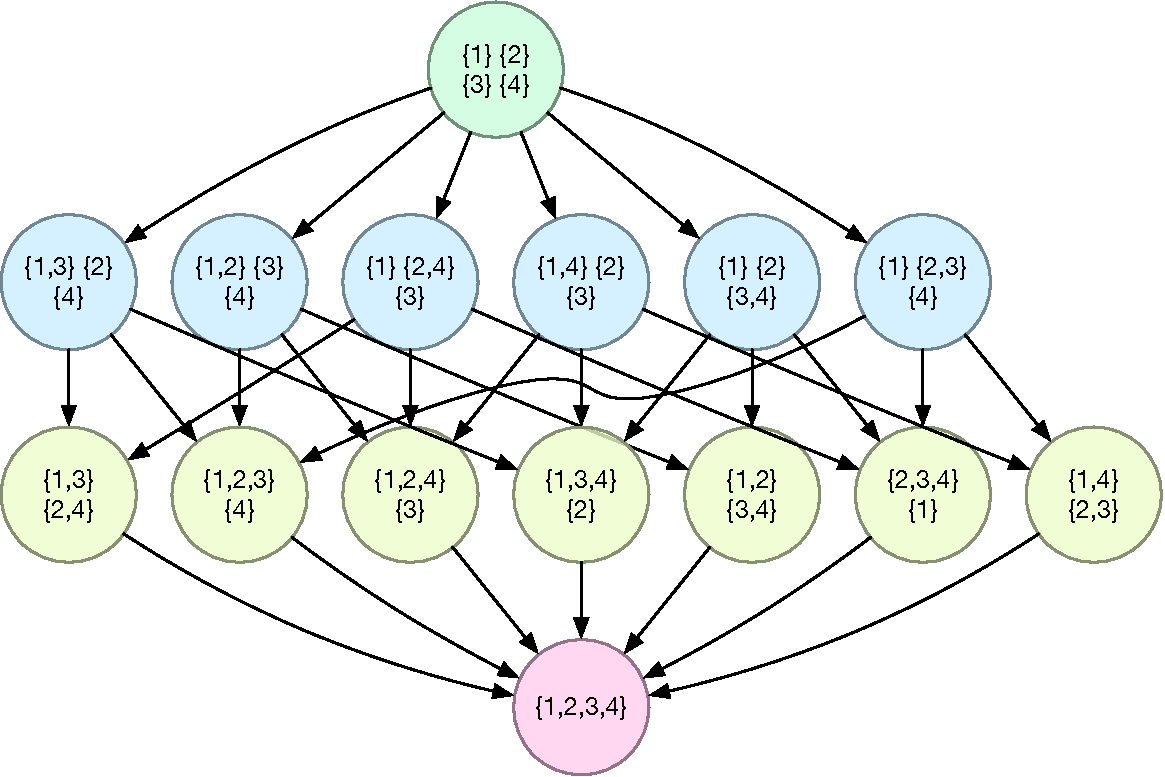
\includegraphics[width=0.7\textwidth]{Chapters/Sequential-coalescent-figures/Transition-system-single-locus}
  \caption{A transition system for the coalescence process that starts with four lineages, 1, 2, 3, and 4. The system moves through states with four, three, two, and one lineage, moving from top to bottom. The left-most path, moving from $\{\{1\},\{2\},\{3\},\{4\}\}$ through $\{\{1,3\},\{2\},\{4\}\}$ and $\{\{1,3\},\{2,4\}\}$ to $\{\{1,2,3,4\}\}$ corresponds to the tree we would write as \texttt{((1,3),(2,4))} in the Newick format.}
  \label{fig:coal-no-recomb-transition-system}
\end{figure}


In a given partition the possible transitions, and the rate at which those transitions can occur, are given only by the set of lineages that the partition consists of. The path through which the system arrived at the partition does not affect the probabilities for choosing the next state to transition to, only the current state. This makes the coalescence process a Markov process, and the way in which transition probabilities are specified makes it an instance of the general class of \emph{continuous time Markov chains}.


\subsection{Continuous time Markov chains}

A (time homogeneous) continuous time Markov chain (CTMC) is a random process $\{\,X(t) \;|\; t \geq 0 \,\}$ where the infinitesimal rate of change between states at time $t$ is given by a \emph{rate matrix} $Q$: Let $\pi(t)$ be the vector of state probabilities $\pi(t)_i = \Pr(X(t)=i)$ then $\frac{\mathrm{d}\,\pi(t)}{\mathrm{d}\,t} = \pi(t)\cdot Q$. The off-diagonal entries of $Q$ contains the rates at which the system changes state, so $Q_{i,j}$ is the rate of change from state $i$ to state $j$, and the diagonal entries are given by $Q_{i,i} = - \sum_{j\neq i} Q_{i,j}$. The probability of going from state $i$ at time $s$ to state $j$ at time $t>s$ in such a system is given by $\Pr(X(t)=j\,|\,X(s)=i) = \left[\exp\left(Q\left(t-s\right)\right)\right]_{i,j}$ and given an initial probability vector $\pi(0)$ the probability vector at time $t\geq 0$ is given by $\pi(t)=\pi(0)\exp(Qt)$.

There is a rich theory for CTMCs so expressing systems in terms of these gives us a very powerful framework to work in. The key property we will use is the way of computing the transition probabilities $\Pr(X(t)=j\,|\,X(s)=i)$ using matrix exponentiation $\exp\left(Q\left(t-s\right)\right)$. This can be done fully automatically---several algorithms exists and matrix exponentiation is implemented in many numerical software packages \cite{Moler2003}---and it greatly simplifies the mathematical modelling---see e.g.\ \citet{Hobolth:2011hl} and \citet{Andersen:2013iz} for examples of where matrix exponentiation simplifies otherwise rather complex computations.

Constructing a CTMC consists of specifying the rate matrix $Q$ and the initial probability vector $\pi(0)$. In most cases this is relatively straightforward, mathematically at least; explicitly specifying the rate matrix can be problematic when the state space is very large. When the state space is large it becomes necessary to automatically generate it and construct the rate matrix. Constructing $Q$ in such cases will be error prone and in most case not practically possible. We will return to automatical construction of CTMCs for coalescence systems in the next chapter.

The coalescence system we considered in the previous section---the simple system with $n$ samples that coalesce at a fixed rate of $c$ per pair of lineages---is easily expressed as a CTMC. We simply need to enumerate all the possible states, i.e.\ all partitions $P\in\partition\left(S\right)$, in order to have indices to use for the matrix and vector. Then, if $\iota$ is the index for the initial partition, we set $\pi(0)_\iota=1$ and $\pi(0)_i=0$ for $i\neq\iota$ and if $P$ and $P'$ are partitions such that there is a transition from $P$ to $P'$, and where $i_P$ and $i_{P'}$ are the indices of those partitions, then $Q_{i_P,i_{P'}}=c$. For all other indices $i$ and $j$, $i\neq j$: $Q_{i,j}=0$, and $Q_{i,i}=-\sum_{j\neq i} Q_{i,j}$.


\subsection{Modelling demographics in the coalescent process}

When we consider the coalescence process as an instance of a continous time Markov chain we immediately have the framework for modelling more complex demographic scenarios. Structured populations, for example, can be modelled by assigning lineages to different populations, allow migration events to move lineages from one population to another, and only allow lineages to coalesce when within the same population. In general, we can extend lineages with any information we wish, and let them undergo any changes we wish, as long as we can model this as a constant rate we can represent in the matrix $Q$.

It is possible to model more complex demographics. A simple example could be to allow the coalescence rate to vary over time. This would capture variation in population size in the population being modelled since, as we recall, the rate is the inverse of the (effective) population size: $c=2/\theta$. A very success full application of this is the PSMC method by \citet{Li:2011ez} that does exactly this through a coalescent hidden Markov model. To model variation in coalescence rate in different time periods we would need a rate matrix for each period. Let $Q^i$ denote the matrix for interval $i: [\tau_i,\tau_{i+1})$. Each $Q^i$ would be constructed as in the previous section but would have a coalescence rate specific to interval $i$: $c_i$.

Since the rate matrix changes over time we cannot simply exponentiate it to get the transition probability matrix when going from time $s$ to time $t$ if $s$ and $t$ are in different time periods, e.g. $s$ in interval $i$ and $t$ in interval $j>i$. If that is the case, however, we can piece together transition probabilities for different intervals. If interval $i$ goes from $\tau_i$ to $\tau_{i+1}$ then the transition matrix for going all the way through interval $i$ is $\exp\left(Q^i(\tau_{i+1}-\tau_i\right)$. Multiplying the transition matrices for two consecutive intervals gives us the probability of going through both:
\begin{multline*}
  \Pr\left(X(\tau_{i+2})=y\,|\,X(\tau_i)=x\right) = \\
   \left[\exp\left(Q^i\left(\tau_{i+1}-\tau_i\right)\right)
         \exp\left(Q^{i+1}\left(\tau_{i+2}-\tau_{i+1}\right)\right)
   \right]_{x,y}
   \quad .
\end{multline*}
With $s$ in interval $i$ and $t$ in interval $j$ we therefore have\begin{multline*}
  \Pr\left(X(t)=y\,|\,X(s)=x\right) = \\
  \left[
      \exp\left(Q^i\left(\tau_{i+1}-s\right)\right)
      \prod_{k=i+1}^{j-1} \exp\left(Q^k\left(\tau_{k+1}-\tau_k\right)\right)
      \exp\left(Q^j\left(t-\tau_j\right)\right)
  \right]_{x,y}
  \quad .
\end{multline*}

We can even construct more complex variation over time, such as merging and splitting populations or turning migration on and off. This, however, often requires combining CTMCs where the state space is different in different time periods which complicates the computations slightly, and we defer a discussion of how to do this to chapters~\ref{chap:composing-CTMCs} and \ref{chap:CTMC-algebra}.


\subsection{The coalescent with recombination}

When also modelling recombination, another type of event is added to the CTMC. Recombination events can take a lineage and split it into two, and the system then continues back in time with these two lineages having independent histories.

Typically this is modelled by having lineages contain so-called ``ancestral material'', which represents the present day samples. Similar to how lineages contained sets of samples when we formulated the model without recombination as a transition system, the ancestral material keeps track of which samples have found a common ancestor. The ancestral material, however, can vary along the sequences.

If we model lineages as consisting of a finite length of nucleotides we can have lineage $x$ represented as $x=(x_1,x_2,\ldots,x_L)$ where each $x_i$ is a subset of the set of samples (for a treatment of the coalescence process with recombination using continous sequences I refer, again, to \citet{Hein:2005vz}). Each $x_i$ plays the role of a single lineage when we modelled the process without recombination; it consists of the samples that have lineage $x$ as a common ancestor at the $i$'th locus. A state of the CTMC will consist of a set of such lineages---and to ensure that this state space is finite we require that for all lineages $x$ at least some $x_i$s are non-empty---such that the $i$'th index sets are disjunct and such that the union of all $i$'th index sets is the full set of samples. We do not require that the $i$'th index sets are partitions of the set of samples; some can be empty sets. Pairs of lineages can coalesce---similar to how it was modelled without recombination---and individual lineages can recombine into two lineages.

A coalescence event would take two lineages, $x=(x_1,\ldots,x_L)$ and $y=(y_1,\ldots,y_L)$, and produce the lineage $z=(x_1\cup y_1,\ldots,x_L\cup y_L)$. A recombination event would take one lineage $x=(x_1,\ldots,x_L)$ and pick a recombination point $k: 1 \leq k < L$. It would then produce two lineages $(x_1,\ldots,x_k,\emptyset,\ldots,\emptyset)$ and $(\emptyset,\ldots,\emptyset,x_{k+1},\ldots,x_L)$ where the ancestral material up to point $k$ is put in the first lineage and the ancestral material after point $k$ is put in the second lineage, and where we would restrict constructed lineages so recombination does not produce lineages without any ancestral material.

A full and formal construction for the process with recombination---for sequences of length two at least but the model generalises easily---is given in chapter~\ref{chap:modelling-2-ARGs}.

The outcome of this process is no longer a tree but a directed acyclic graph called the \emph{ancestral recombination graph} or ARG, see Figure~\ref{fig:ARG-and-local-genealogies}, A). While not a tree itself, the ARG represents a set of trees since at each position along the sample sequences a single tree describes the genealogy at that position, see Figure~\ref{fig:ARG-and-local-genealogies}, B). At positions where a recombination has occurred the tree to the left and to the right of the recombination position can be different. The probability density over all possible ARGs thus also provides a joint probability for all the corresponding local tree-genealogies.

\begin{figure}
 \center
    \begin{subfigure}[t]{0.41\textwidth}
        \centering
        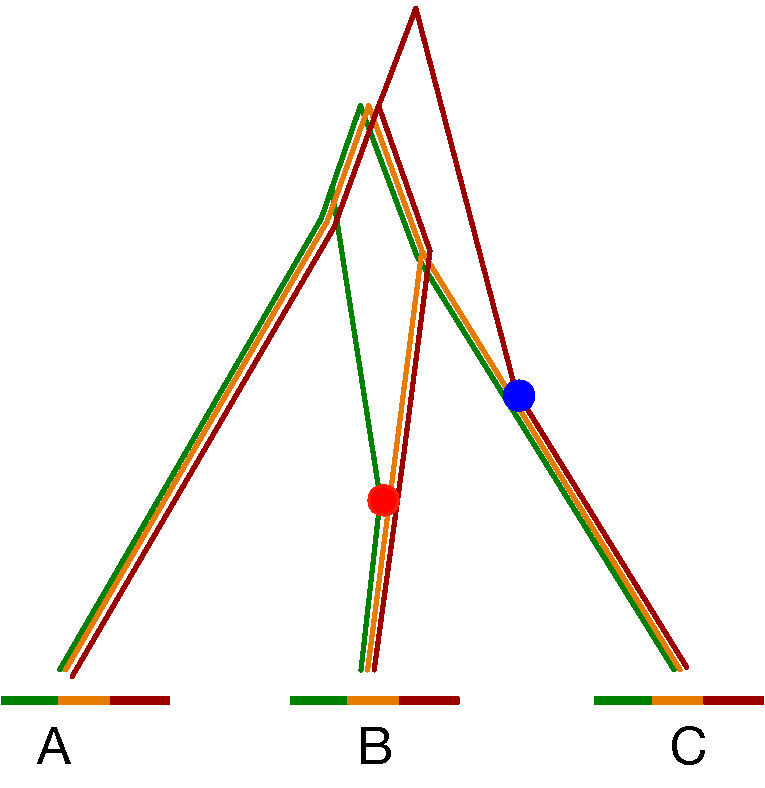
\includegraphics[width={0.9\textwidth}]{Chapters/Sequential-coalescent-figures/ARG}
        \caption{An ancestral recombination graph over three sequences, showing two recombinations.}
    \end{subfigure}%
    ~ 
    \begin{subfigure}[t]{0.55\textwidth}
        \centering
        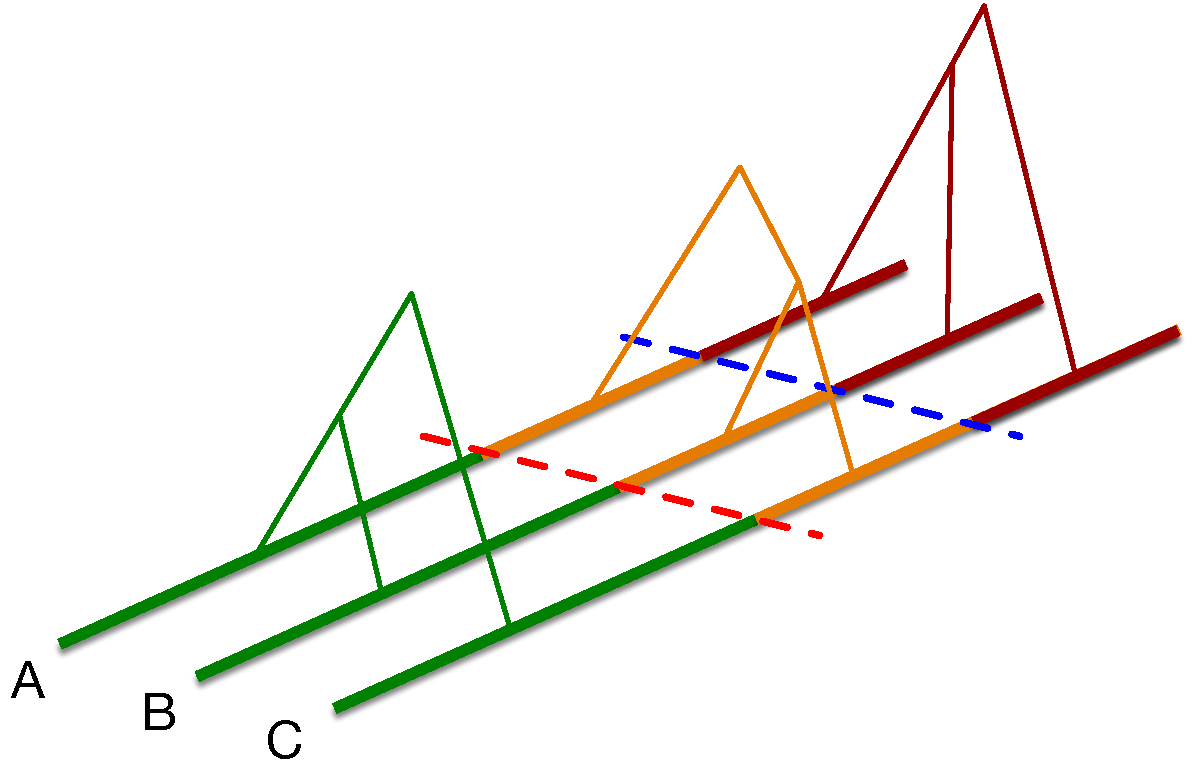
\includegraphics[width={0.9\textwidth}]{Chapters/Sequential-coalescent-figures/Local-genealogies}
        \caption{The corresponding three local genealogies.}
    \end{subfigure}%
  \caption{The example shows the ancestry of three sequences in the case where they have experienced two recombination events, shown in red and green. These recombinations segments the sequences into three regions, shown in blue, orange and purple, each with different tree genealogies.}
  \label{fig:ARG-and-local-genealogies}
\end{figure}

There is not a one-to-one correspondence between the local genealogies and the ARG: different ARGs can have exactly the same local genealogies. This is obvious when considering that the timing of recombination events cannot be seen in the local trees. Even ignoring the timing of events there is not a one-to-one correspondence between ARG topologies and the local trees: different ARGs can have the same local trees if recombined lineages coalesce back together in such a way that the local trees do not change. If, for example, a lineage recombines and the two resulting lineages coalesce back again before coalescing with other lineages, this form a ``diamond'' shape in the ARG that is invisible in the local trees. For the purpose of this thesis this is a subtlety we will mostly ignore.

We will be interested in the ARG as a means to generating local trees only and whenever possible either integrate over all ARGs generating the same local trees or even integrate over all ARGs generating the same sequences.


\subsection{Mutations and the likelihood of sampled sequences}

Mutations on lineages can also be considered events in the CTMC, which can occur and modify lineages as the process runs back in time, but typically mutations are put on the coalescence tree or ARG after it is simulated. There, the mutations can simply be put on the genealogy as a Poisson process or be put on inner nodes using a substitution model. The latter approach makes it possible to sum over all possible sequences at internal nodes using standard methods such as Felsenstein's peeling algorithm \cite{Felsenstein_1981} and this way obtain a joint probability distribution for the sequences at the leaves, i.e.\ the present day samples. This distribution depends only on the local tree-genealogies induced by the ARG since the possible nucleotides at any given position only depends on the tree for that given position.

If we denote by $\Theta$ the relevant parameters for the coalescence process, e.g. coalescence rates, migration rates, recombination rates, and mutation rates, we can let $f(\G\,|\,\Theta)$ denote the probability density for the process producing the specific genealogy $\G$ and let $f(\A\,|\,\G,\Theta)$ denote the probability that putting mutations on genealogy $\G$ produces the aligned samples $\A$. Typically the alignment probabilities only depends on the mutation rate while the genealogy probabilities is independent of the mutation rate but depends on the coalescence process CTMC and its parameters such as rates (migration, recombination etc.) and time points where it switches between different rate matrices or state spaces.

For demographic inference it is the parameters in $\Theta$ that are of interest rather than the actual underlying genealogy, which is considered a nuisance parameter to be integrated out to get the likelihood
\[
    \lhd(\Theta\,|\,\A) = \int f(\A\,|\,\G) f(\G\,|\,\Theta) \intd\G .
\]

This integral over all possible genealogies is generally not efficiently computable and must either be approximated through sampling approaches or by approximating the coalescence process with a simpler model where the integral \emph{can} be computed. 

In other cases we are interested in inferring the most probable genealogy given the sequence alignment and a fixed set of parameters
\begin{displaymath}
  \argmax_\G f(\G\,|\,\A,\Theta) = 
  \argmax_\G f(\A\,|\,\G) f(\G\,|\,\Theta)
  .
\end{displaymath}

Both of these inference problems can be efficiently solved if we approximate ARG as a sequential Markov process: a coalescence hidden Markov model.

\section{Coalescence hidden Markov models}

The key approximation in coalescence hidden Markov models, or CoalHMMs, is assuming that the distribution of local genealogies along an alignment is Markov. This means that when moving from one tree to another across a recombination point, the next tree depends only on the current tree and not any others. 

By approximating the distribution of local genealogies by a Markov chain the probability of the full genealogy reduces to specifying the joint probability of two neighbouring genealogies (which might be identical genealogies, e.g.\ if there is no recombination between them). Let $\ell$ denote the ``left'' genealogy and $r$ the ``right'' genealogy and $T_\Theta(r \,|\, \ell)$ the ``transition density''. If our data $\A$ consists of $L$ nucleotides then the underlying genealogy $\G=\G_1,\G_2,\ldots,\G_L$  consists of $L$ local trees (where some can be identical) and
\[
    f(\G\,|\,\Theta) = p_\Theta(\G_1) \prod_{i=2}^L T_\Theta(\G_i\,|\,\G_{i-1}) .
\]

The alignment probability given these local genealogies separates into probabilities for the individual nucleotides so if $\A_i$ denotes the $i$'th column in the alignment then
\[
    f(\A\,|\,\G) = \prod_{i=1}^L E_\Theta(\A_i\,|\,\G_i) .
\]
where $E_\Theta(\A_i\,|\,\G_i)$---the ``emission probability''---is the probability that the $\A_i$ column was produced by tree $\G_i$ and can be computed using the peeling algorithm.

In order to integrate over all genealogies we further approximate by discretising the possible time points where inner nodes can be found in the trees. We split the possible coalescence times into $n$ intervals and place all events in the same interval at a single time point. If $p_\Theta(\ell)$ denotes the probability that the left-most tree has the genealogy $\ell$ then we can sum over all possible genealogies
%\begin{equation}
%    \label{eq:integrating-over-genealogies}
%    \begin{split}
%    &\int f(\A\,|\,\G) f(\G\,|\,\Theta) \intd\G =\\
%    &\sum_{\G_1,\ldots,\G_L} \left[ 
%        p_\Theta(\G_1) E(\A_1\,|\,\G_1) 
%        \prod_{i=2}^L T_\Theta(\G_i\,|\,G_{i-1}) E(\A_i\,|\,\G_i)
%    \right] .
%    \end{split}
%\end{equation}
\begin{dmath}
    \label{eq:integrating-over-genealogies}
    \int f(\A\,|\,\G) f(\G\,|\,\Theta) \intd\G = \\
    \sum_{\G_1,\ldots,\G_L} \left[ 
        p_\Theta(\G_1) E(\A_1\,|\,\G_1) 
        \prod_{i=2}^L T_\Theta(\G_i\,|\,G_{i-1}) E(\A_i\,|\,\G_i)
    \right] .
\end{dmath}

This equation takes the form of a hidden Markov model \cite{Rabiner_1989}, where the sequence $\A_1,\ldots,\A_L$ is the observable sequence and $\G_1,\ldots,\G_L$ the hidden Markov sequence.

\subsection{Hidden Markov models}

There is an exponential number of genealogies to sum over in equation \eqref{eq:integrating-over-genealogies}. If there is $N$ possible genealogies local genealogies---genealogies for single loci---and the sequence is $L$ loci long, then the sum is over $N^L$ different sequences of local genealogies. We can rearrange the sum, however, and by applying dynamic programming, the likelihood can be computed in running time $O(N^2L)$.

The algorithm for computing \eqref{eq:integrating-over-genealogies} using dynamic programming is known as the \emph{Forward} algorithm and is part of a suite of algorithms for efficient inference in the framework known as hidden Markov models~\cite{Rabiner_1989,Durbin:2005wq}.

A \emph{hidden Markov model} (HMM) with $N$ ``hidden states'' and $M$ ``observable states'' is defined by a triplet $(T,E,p)$ where $T$ is an $N\times N$ probability matrix (entries are non-negative and rows sum to one), $E$ is an $N\times M$ probability matrix, and $p$ is a $1\times N$ probability vector.

When modelling the ancestry of samples, the hidden states are the local genealogies---that cannot be directly observed---and the observable states are the alignment columns---that \emph{can} be directly observed.

The $p$ vector specifies the probability of starting the hidden sequence in a given state. If $H=(H_1,H_2,\ldots,H_L)$ is a stochastic sequence of hidden states, then $\Pr(H_1=h_1)=p_{h_1}$. The transition matrix, $T$, captures the probabilities for moving through a sequence of hidden states as a Markov process:
\(
    \Pr(H=(h_1,h_2,h_3,\ldots,h_L)) =
    p_{h_1} \cdot \prod_{i=2}^L T_{h_{i-1},h_i}
\). The emission matrix, $E$, specifies the probability of observing state $o_i$ at index $i$ conditional on the hidden state $h_i$ at index $i$: If $O=(O_1,O_2,\ldots,O_L)$ is a stochastic sequence of observable states then 
\(
    \Pr(O=(o_1,\ldots,o_L)\,|\,H=(h_1,\ldots,h_L)) = \prod_i E_{h_i,o_i}
    .
\)

The joint probability of observing both the hidden and the observed sequence is given by
\begin{dmath*}
  \Pr\left(H=(h_1,\ldots,h_L), O=(o_1,\ldots,o_L)\right) =
  p_{h_1} E_{h_1,o_1} \prod_{i=2}^L T_{h_{i-1},h_i} E_{h_i,o_i}
\end{dmath*}
which has the form of the expression inside the sum of equation~\eqref{eq:integrating-over-genealogies}, and not surprisingly the probability of seeing just the observable sequence is
\begin{dmath*}
  \Pr\left(O=(o_1,\ldots,o_L)\right) =
  \sum_{H} \left[
      p_{h_1} E_{h_1,o_1} \prod_{i=2}^L T_{h_{i-1},h_i} E_{h_i,o_i}
  \right]
\end{dmath*}
exactly as equation~\eqref{eq:integrating-over-genealogies}.

The link between the hidden Markov model specification and the coalescence genealogy and alignment probabilities should be obvious: the initial probability vector $p$ is the probability of observing a given genealogy
\begin{dmath*}
    p_i = p_\Theta(\G_i)
\end{dmath*}
the emission matrix is the probability of seeing the alignment column $\A_j$ given the genealogy $G_i$
\begin{dmath*}
    E_{i,j} = E(\A_j\,|\,\G_i)
\end{dmath*}
and the transition probabilities are just
\begin{dmath*}
    T_{i,j} = T_\Theta(\G_j\,|\,\G_i)
    \ .
\end{dmath*}

\subsection{Inference in hidden Markov models}

There is a suite of algorithms for working with hidden Markov models. A thorough treatment of these is beyond the scope of this text but three are worth sketching here: how to compute the likelihood of the parameters given only an observed sequence, how to compute the most probable sequence of hidden states, and how to compute the most probable local genealogy for a given index. These are know as the \emph{Forward} algorithm, the \emph{Viterbi} algorithm, and the \emph{Posterior Decoding}, respectively.

For ease of notation we will use $X_{i:j}$ to mean $(X_i,X_{i+1},\ldots,X_{j})$, i.e.\ the subsequence from $i$ to $j$, for sequences $X$.

\paragraph{The Forward algorithm}

Given a sequence of observable states $o_{1:L}$, the Forward algorithm computes a table of joint probabilities:
\begin{displaymath}
  F[i,h] = \Pr\left(H_i=h, O_{1:i}=o_{1:i}\right)
\end{displaymath}
i.e.\ the table entry $F[i,h]$ contains the probability of observing the prefix of the observed sequence $o_{1:i}$ and being in hidden state $h$ at step $i$. (The probability here is conditional on the three parameters $p$, $T$, and $E$, of the hidden Markov model, but since all probabilities in this section will depend on the same parameters we leave this implicit). This probability is, by the law of total probability, equal to
\begin{equation}
    \label{eq:forward-sum}
  F[i,h] = 
  \sum_{h_{1:i-1}}
  \Pr\left(H_{1:i-1}=h_{1:i-1}, H_i=h, O_{1:i}=o_{1:i}\right)
\end{equation}
which we can rephrase recursively as
\begin{dmath*}[breakdepth=-1]
  F[i,h] 
    =
     \sum_{h_{i-1}}
      \Pr\left(H_i\hiderel{=}h, O_i\hiderel{=}o_i \,|\, H_{i-1}\hiderel{=}h_{i-1}\right)
      \\\quad\times
      \sum_{h_1,\ldots,h_{i-2}}
          \Pr\left(H_{1:i-1}\hiderel{=}h_{1:i-1}, O_{1:i-1}\hiderel{=}o_{1:i-1}\right)
    =
      \sum_{h_{i-1}}
      \Pr\left(H_i\hiderel{=}h, O_i\hiderel{=}o_i 
               \,|\,
               H_{i-1}\hiderel{=}h_{i-1}\right)
             F[i-1,h_{i-1}] 
    =
      \sum_{h_{i-1}} E_{h,o_i} T_{h_{i-1},h} F[i-1,h_{i-1}]
\end{dmath*}
with the special case for $i=1$:
\begin{displaymath}
  F[1,h] = p_h \cdot E_{h,o_1}
  .
\end{displaymath}

Computing the value in each cell takes time $N$---for the sum in the recursion---and there are $N\times L$ cells in the table, so the entire table can be computed in time $O(N^2L)$. Since $F[L,h]$ is the probability of seeing the entire observable sequence and then being in hidden state $h$ we can get the probability of just seeing the observable sequence---applying again the law of total probability---as $\Pr(O)=\sum_h F[L,h]$. This is the likelihood of the observed sequence given the HMM parameters, and the parameters can be estimated by maximising this likelihood.

If we are only interested in the actual sequence likelihood and not the full table, some shortcuts and heuristics can be used to speed up the computations. The algorithm in \citet{Sand:2013bi}, for example---the one we use in likelihood optimisations in the Python framework where we implement our CoalHMMs---exploits that genome alignments consist of very repetitive sequences and preprocess the alignment into a structure where the likelihood can be computed very efficiently.


\paragraph{The Viterbi algorithm}

Instead of computing the probability of the observed sequence, $\Pr(O)=\sum_{H}\Pr(H,O)$, the Viterbi algorithm computes the most probable hidden sequence: $\argmax_H \Pr(H,O)$, (or one such sequence if there are more with the same probability).

The first part of the algorithm follows the Forward algorithm very closely and fills in a table, but for the Viterbi algorithm the table contains the maximum over all possible hidden paths ending in state $h$ rather than the sum over all of them:
\begin{displaymath}
  V[i,h] = 
  \max_{h_{1:i-1}} \Pr\left(H_{1:i-1}=h_{1:i-1}, H_i=h, O_{1:i}=o_{1:i}\right)
\end{displaymath}
and the recursion for computing is identical to the recursion in the Forward algorithm except that maximum is used instead of sum.

Once this table is computed---which like the Forward algorithm can be done in time $O(N^2L)$---we can find the last state in the most likely hidden path as the state $h_L = \argmax_h V[L,h]$ (or one such state if there are ties). From this state we can backtrack the HMM transitions to read off the most likely path.

The most likely second last state is not necessarily the state $h$ that maximises $V[L-1,h]$ since a transition from that state to $h_L$ could potentially be very unlikely. The most likely state at index $L-1$ must be the state $h_{L-1}$ that satisfy $V[L-1,h_{L-1}] T_{h_{L-1},h_L} E_{h_L,o_L} = V[L,h]$ (or an arbitrary such if there are more than one). This state satisfy that, if we have the best possible path that ends in $h_{L-1}$ then taking one more step, to the final state $h_L$, we will have an optimal path (since $h_L$ was selected to be optimal). Scanning through row $L-1$ in $V$ we can thus find the second-last state in the optimal path. We can then repeat this for the third-to-last state and so forth until we have read off the complete optimal hidden path.

In this backtracking phase of the algorithm we need to scan through $N$ states for each of the $L$ positions so the running time is $O(NL)$.


\paragraph{Posterior Decoding}

The Posterior Decoding algorithm calculates the probability of seeing a given hidden state, $h$, at a given position, $i$, conditional on the entire observed sequence: $\Pr(H_i=h\,|\,O=o)$. This can be done for all indices $i$ at the same complexity as computing it for a single index. From this we can read off the most likely hidden state for each position along the sequence, but keep in mind that a sequence of most likely states at each position does not necessarily combine to a most likely complete sequence---or for that matter even a possible sequence.

The posterior probability for seeing state $h$ at position $i$ given the observable sequence $O=o$ can be written as 
\begin{displaymath}
    \Pr(H_i=h\,|\,O=o) = \frac{\Pr(H_i=h,O=o)}{\Pr(O=o)},
\end{displaymath}
where the value $\Pr(O=o)$ is the likelihood we compute with the Forward algorithm, and we have
\begin{dmath*}
    \Pr(H_i=h,O=o) = \\
        \sum_{h_{1:i-1}, h_{i+1:L}} 
        \left.
            \Pr(H_i=h, H_{1:i-1}=h_{1:i-1}, H_{i+1:L}=h_{i+1:L},O=o) 
        \right.
\end{dmath*}
by the law of total probability.

We can further break this up into the sequences before and after position $i$---exploiting along the way that $O_i$ only depends on $H_i$ and not the full hidden sequence---to get
\begin{dmath*}
    \Pr(H_i=h,O=o) = \\
    \sum_{h_{1:i-1}}
    \left.
        \Pr(H_i=h, H_{1:i-1}=h_{1:i-1},O_{1:i}=o_{1:i})
    \right.
    \times 
    \left.
        \sum_{h_{i+1:L}} \Pr(H_{i+1:L}=h_{i+1:L}, O_{i+1:L}=o_{i+1:L}\,|\,H_i=h)
    \right.
\end{dmath*}

The first part of this is the value we compute using the Forward algorithm
\begin{displaymath}
    F[i,h] = \sum_{h_{1:i-1}} \Pr(H_i=h, H_{1:i-1}=h_{1:i-1},O_{1:i}=o_{1:i})
\end{displaymath}
(see eq.~\eqref{eq:forward-sum}), and we can define
\begin{dmath}
\label{eq:backward-sum}
  B[i,h] = 
  \sum_{h_{i+1:L}} 
      \left.\Pr\left(H_{i+1:L}=h_{i+1:L}, O_{i+1:L}=o_{i+1:L}\,|\,H_i=h\right)\right.
  = \left.\Pr\left(O_{i+1:L}=o_{i+1:L}\,|\,H_i=h\right)\right.
\end{dmath}
to get
\begin{displaymath}
  \Pr(H_i=h,O=o) = F[i,h] \cdot B[i,h].
\end{displaymath}

The table $B[i,h]$ defined in eq.~\eqref{eq:backward-sum} can be computed using dynamic programming---very similarly to the table $F[i,h]$---by an algorithm called the Backward algorithm. Both tables $F[i,h]$ and $B[i,h]$ can be computed in time $O(N^2L)$ and after that the posterior distribution at each index can be read off in time $O(N)$.


\subsection{Constructing transition probabilities}

The crux of constructing a CoalHMM---and thereby getting access to the hidden Markov model algorithms for inference---is specifying the probability of transitioning from one local genealogy to another: That is, constructing the transition probability matrix of the hidden Markov model, as a function of the parameters of the coalescence CTMC we aim to approximate. Once this transition matrix is constructed we can obtain the the initial probabilities $p_\Theta$ from marginalisation and the emission probabilities using standard algorithms.

In the literature there are two approaches to computing this transition matrix. Either it is computed by conditioning on the current tree, placing a recombination point on it, and tracking where it can re-coalesce~\cite{Hobolth:2014cw,Li:2011ez} or it is computed by considering the joint distribution of two neighbouring trees~\cite{Dutheil:2009dt,Mailund:2011dv}. The latter is the approach we will consider in this thesis.

Let $J_\Theta(\ell,r)$ denote the joint probability of seeing the genealogy $\ell$ on the left and $r$ on the right of two nucleotides. Then the transition probability is given by
\[
    T_\Theta(r \,|\, \ell) = \frac{J_\Theta(\ell,r)}{p_\Theta(\ell)}
\]
and the initial probabilities given by
\[
    p_\Theta(\ell) = \sum_{r} J_\Theta(\ell, r)
    .
\]

The probabilities $J_\Theta(\ell,r)$ can be computed using continuous time Markov chains tracking the ancestry of two neighbouring nucleotides, which is the topic of the following chapters.
